\documentclass[11pt,a4paper]{article}
\usepackage[latin1]{inputenc}
\usepackage[dutch]{babel}
\usepackage{graphicx}
\usepackage{amssymb}
\usepackage{hyperref}
\usepackage{amsmath}
\usepackage{caption}
\usepackage{subcaption}

\author{Dieter Decaestecker, Sander Demeester, Tom Naessens, Nick Van Haver}
\title{Verslag Project Datacommunicatie}
\date{21 december 2012}
\parindent 0pt
\hypersetup{
    colorlinks,
    citecolor=black,
    filecolor=black,
    linkcolor=black,
    urlcolor=black
}

\begin{document}
\maketitle
\tableofcontents


\section{Broncodering}

Het grafische bestand dat wij zullen gebruiken voor het illustreren van de broncodering is het bestand `alberteinstein.bmp'.

\subsection{Opstellen Huffmancode}
\subsubsection{Relatieve frequenties}
% Bijvoegen file 1.1.m
De matlab code voor deze opgave staat in het bestand \texttt{1.1.m} in de bijgeleverde files. Het resultaat hiervan is te zien in tabel \ref{tab:1.1}. De bijbehorende Huffmancode die we met deze frequenties bekomen is terug te vinden in tabel \ref{tab:1.2} op pagina \pageref{tab:1.2}.

\begin{table}
\centering
\begin{tabular}{c|c|r|c}
Nummer & Macrosymbool & Abs. Freq. & Rel. Freq. \\ 
\hline 
1 & \begin{tabular}{cc}$\square$ & $\square$ \\ $\square$ & $\square$ \end{tabular} & 12478 & 0.407777777777778 \\ 
\hline 
2 & \begin{tabular}{cc}$\square$ & $\square$ \\ $\square$ & $\blacksquare$\end{tabular} & 193 & 0.006307189542484 \\ 
\hline 
3 & \begin{tabular}{cc}$\square$ & $\blacksquare$ \\ $\square$ & $\square$\end{tabular} & 172 & 0.005620915032680 \\ 
\hline 
4 & \begin{tabular}{cc}$\square$ & $\blacksquare$ \\ $\square$ & $\blacksquare$\end{tabular} & 227 & 0.007418300653595 \\ 
\hline 
5 & \begin{tabular}{cc}$\square$ & $\square$ \\ $\blacksquare$ & $\square$\end{tabular} & 168 & 0.005490196078431 \\ 
\hline 
6 & \begin{tabular}{cc}$\square$ & $\square$ \\ $\blacksquare$ & $\blacksquare$\end{tabular} & 235 & 0.007679738562092 \\ 
\hline 
7 & \begin{tabular}{cc}$\square$ & $\blacksquare$ \\ $\blacksquare$ & $\square$\end{tabular} & 18 & 0.000588235294118 \\ 
\hline 
8 & \begin{tabular}{cc}$\square$ & $\blacksquare$ \\ $\blacksquare$ & $\blacksquare$\end{tabular} & 147 & 0.004803921568627 \\ 
\hline 
9 & \begin{tabular}{cc}$\blacksquare$ & $\square$ \\ $\square$ & $\square$\end{tabular} & 194 & 0.006339869281046 \\ 
\hline 
10 & \begin{tabular}{cc}$\blacksquare$ & $\square$ \\ $\square$ & $\blacksquare$\end{tabular} & 8 & 0.000261437908497 \\ 
\hline 
11 & \begin{tabular}{cc}$\blacksquare$ & $\blacksquare$ \\ $\square$ & $\square$\end{tabular} & 269 & 0.008790849673203 \\ 
\hline 
12 & \begin{tabular}{cc}$\blacksquare$ & $\blacksquare$ \\ $\square$ & $\blacksquare$\end{tabular} & 157 & 0.005130718954248 \\ 
\hline 
13 & \begin{tabular}{cc}$\blacksquare$ & $\square$ \\ $\blacksquare$ & $\square$\end{tabular} & 175 & 0.005718954248366 \\ 
\hline 
14 & \begin{tabular}{cc}$\blacksquare$ & $\square$ \\ $\blacksquare$ & $\blacksquare$\end{tabular} & 99 & 0.003235294117647 \\ 
\hline 
15 & \begin{tabular}{cc}$\blacksquare$ & $\blacksquare$ \\ $\blacksquare$ & $\square$\end{tabular} & 173 & 0.005653594771242 \\ 
\hline 
16 & \begin{tabular}{cc}$\blacksquare$ & $\blacksquare$ \\ $\blacksquare$ & $\blacksquare$\end{tabular} & 15887 & 0.519183006535948 \\
\end{tabular} 
\caption{Weergave nummers t.o.v. macrosymbolen samen met hun absolute en relative frequentie}
\label{tab:1.1}
\end{table}


\begin{table}
\centering
\begin{tabular}{c|l}
Nummer & Huffmancode \\
\hline
1 & 10\\
\hline
2 & 110000\\
\hline
3 & 110011\\
\hline
4 & 11110\\
\hline
5 & 110100\\
\hline
6 & 11101\\
\hline
7 & 11011110\\
\hline
8 & 110110\\
\hline
9 & 11111\\
\hline
10 & 11011111\\
\hline
11 & 11100\\
\hline
12 & 110101\\
\hline
13 & 110001\\
\hline
14 & 1101110\\
\hline
15 & 110010\\
\hline
16 & 0\\
\end{tabular} 
\caption{Weergave nummers van de macrosymbolen met hun corresponderende Huffmancode}
\label{tab:1.2}
\end{table}

\subsubsection{Resulterende Huffmanboom}

In figuur \ref{fig:1.huff} op pagina \pageref{fig:1.huff} staat de boom die we bekomen door de Huffmancode uit tabel \ref{tab:1.2} te visualiseren. Hier hebben we aan de takken naar de grootste van de twee probabiliteiten (de opwaardse tak) het 0 bit toegekend. De andere takken krijgt dus het bit 1 toegekend. Ter controle hebben we ook de probabiliteiten van de tussenliggende knopen opgenomen in de boom.

\begin{figure}[h!]
  		\centering
   		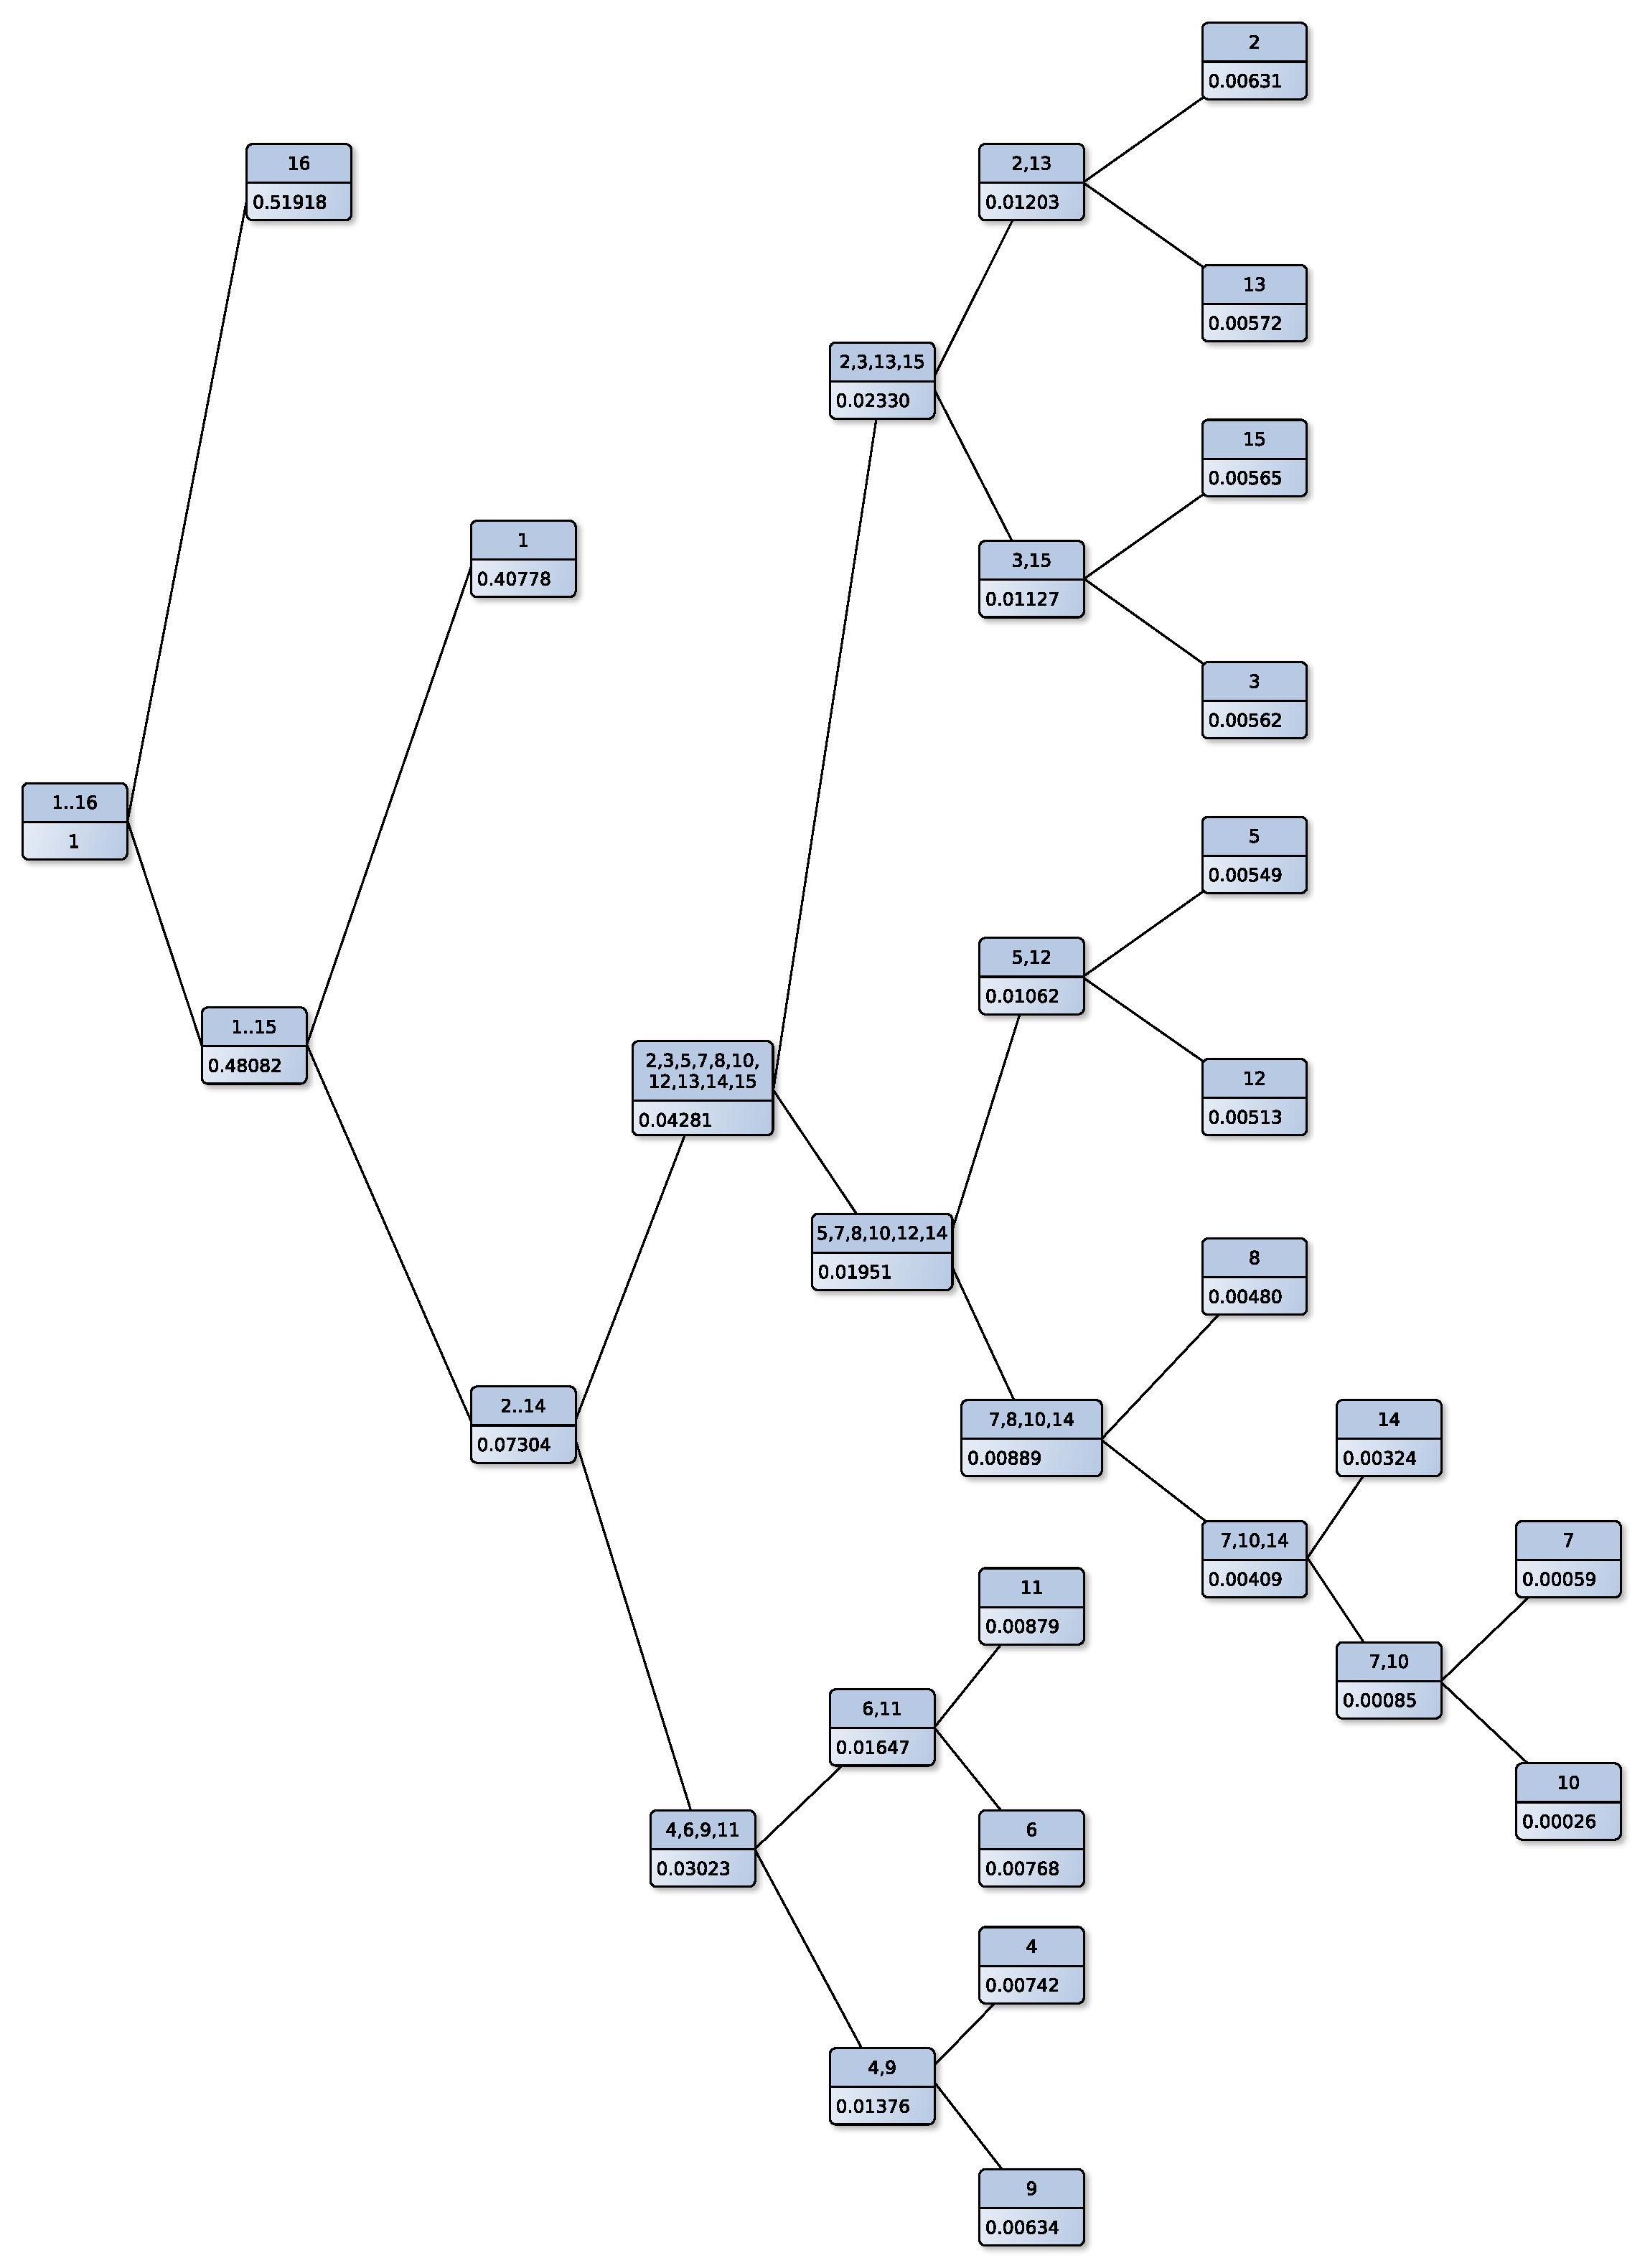
\includegraphics[width=1.1\textwidth]{1_1_huffman_tree.pdf}
  	  	\caption{Huffmanboom voor Huffmancode uit tabel \ref{tab:1.2}}
  		\label{fig:1.huff}
\end{figure}

\subsubsection{Gemiddeld aantal codebits}

Het gemiddelde aantal codebits per bronsymbool berekenen we met volgende formule uit de cursus.
\begin{equation}
E[n]=\frac{1}{K} \sum_{i=1}^{N} p_i n_i
\end{equation}
In deze formule is K het aantal bronsymbolen per macrosymbool, N het aantal verschillende macrosymbolen, $p_i$ de kans om codewoord $c_i$ te bekomen en $n_i$ de lengte van het codewoord $c_i$. In ons geval hebben we dus dat K = 4, N = 16, $p_i$ zijn de probabiliteiten uit tabel \ref{tab:1.1} en $n_i$ de lengte van de codewoorden uit tabel \ref{tab:1.2}. Als we deze formule uitwerken, bekomen we een gemiddeld aantal codebits $E[n]$ van afgerond 0.44 bits per bronsymbool. We zullen per pixel dus gemiddeld slechts 0.4 bits nodig hebben.

\subsection{Implementatie \texttt{create\_codebook$\left(\right)$}}

De implementatie van deze funtie is terug te vinden in het bestand \texttt{Source\_Coding.m}. Deze functie maakt ook gebruik van het node-object, terug te vinden in \texttt{node.m}.\\\\
De functie is als volgt ge\"implementeerd: Eerst wordt een array opgesteld van node-objecten, met elk zijn letter en frequentie. Daarna sorteren we deze array op frequentie en voegen we de twee laatste nodes samen door deze het linker- en rechterkind te maken van een oudernode. Deze oudernode wordt dan terug achteraan de array toegevoegd. Dit herhalen we tot er nog 1 element in deze array zit; de wortel.\\\\
Daarna doorlopen we onze boom vanuit de wortel naar de bladeren en stellen we stapsgewijs de code op. Telkens we in een blad komen voegen we de huidige code toe aan de codewordsarray. Eenmaal we alle bladeren gehad hebben geven we deze array terug als resultaat.\\
Meer codegerelateerd commentaar is bijgevoegd in de codebestanden.

\subsection{Entropie (K = 1..10)}

De entropie corresponderend met de frequenties van het bestand \texttt{`Xfile4.mat'} bekomen we met het script \texttt{1.3.m}. Hierin maken we gebruik van volgende formule uit de cursus:
\begin{equation}
H(X)=-\sum_{x \in A} p(x) log_2(p(x))
\end{equation}

Hier is $X$ de toevalsveranderlijke, p(x) is de kans dat $X=x$, dus dat we een bepaald macrosymbool hebben. $A$ is de verzameling van alle mogelijke macrosymbolen. De plot voor deze entropie voor een aantal K samengenomen bronssymbolen is te zien in figuur \ref{fig:1.3_entropie} op pagina \pageref{fig:1.3_entropie}.\\

\begin{figure}[h!]
  		\centering
   		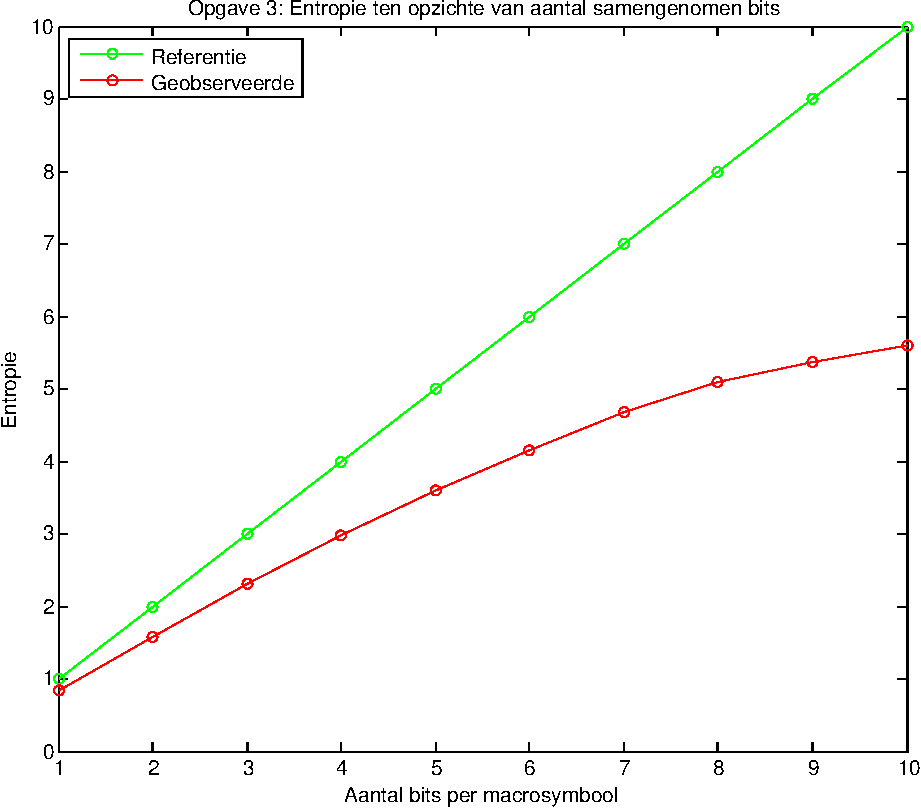
\includegraphics[width=0.8\textwidth]{1_3_entropie.pdf}
   		\caption{Entropie t.o.v. aantal samengenomen bits}
  		\label{fig:1.3_entropie}
\end{figure}

We zien dat de entropie voor de frequenties van de afbeelding eerder logaritmisch stijgt ten opzichte van de referentie die lineair stijgt. Hierdoor zal de entropie voor grotere waarden van K verder afwijken van de referentie. We zien geen duidelijke waarde die beter is dan de andere. We moeten dus een afweging maken van de complexiteit ten opzichte van de entropie. Bij te grote waarden voor K krijgen we immers het probleem dat de berekening te complex wordt.  

\subsection{Gemiddeld aantal codebits (K = 1..10)}

Het gemiddelde aantal codebits per bronsymbool hebben we berekend aan de hand van script \texttt{`1.4.m'}. Als bovengrens en ondergrens hebben we respectievelijk de entropie $H(X)$ en $H(X)+\frac{1}{K}$. We zien dat het gemiddeld aantal codebits al bij macrosymbolen van grootte 3 al zeer dicht bij de ondergrens aanligt. Om een bestand optimaal te comprimeren zijn twee zaken belangrijk: enerzijds willen we na het comprimeren een zo klein mogelijk bestand en anderzijds willen we ook dat het en- en decoderen niet t\'e veel tijd in beslag neemt. Het samennemen van meer bits voor de macrosymbolen zal leiden tot een kleiner bestand, maar zal ook leiden tot een langere decodeertijd.\\
Als we kiezen voor een zo klein mogelijk gecomprimeerd bestand dan kiezen we best voor een aantal samengenomen bits van 10. Zo krijgen we een optimaal gecomprimeerd bestand.\\
Als we echter willen kiezen voor een zo snel mogelijke decompressie kiezen we beter voor een lager aantal bits die toch nog steeds dicht bij de ondergrens aansluit zoals 3.\\
Uiteindelijk kiezen we voor een compromis tussen beide, dat iets zwaarder zal doorwegen naar een meer optimale compressie aangezien dit hier belangrijker is. We kiezen uiteindelijk om 8 bits samen te nemen per macrosymbool.\\

De compressiefactor komt overeen met de effici\"entie van de code. Deze effici\"entie kunnen we aflezen uit figuur \ref{fig:1.4_E} op pagina \pageref{fig:1.4_E}. Voor de compressie zal het bestand een grootte hebben van 55440 bits. Na de compressie zal dit bestand, met een optimale aantal samengenomen bits (namelijk 10 bits) slechts 31323 bits innemen.  We hebben dus een compressiefactor van $\frac{31323}{55440} = 0.564989177$\%.\\
Met een suboptimaal aantal samengenomen bits (namelijk 8) verkrijgen we een compressiefactor van $\frac{35605}{55440} = 0.64222583$\%.

\begin{figure}[h!]
  		\centering
   		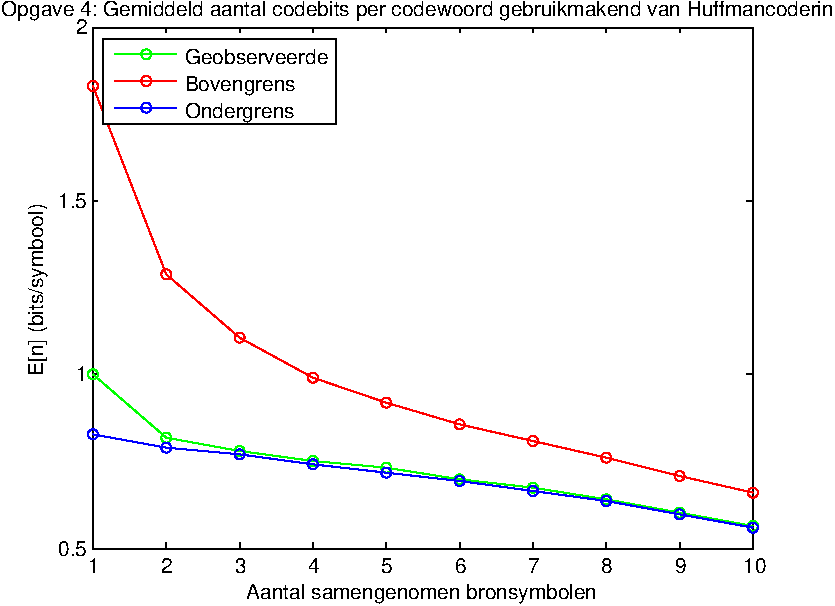
\includegraphics[width=0.8\textwidth]{1_4_E.pdf}
  		\caption{Gemiddeld aantal codebits per codewoord bij Huffmancodering}
  		\label{fig:1.4_E}
\end{figure}

\subsection{Bespreking E[n] tegenover ondergrens}

Zoals we zien op figuur \ref{fig:1.4_E} op pagina \pageref{fig:1.4_E} zien we dat het gemiddeld aantal bits per bronsymbool al zeer snel in de buurt komt van de ondergrens. We zien dus dat we een hele effici\"ente code hebben. Exact de ondergrens bereiken is theoretisch mogelijk; ten eerste moet onze gekozen K 'oneindig' zijn, wat in de praktijk overeenkomt met K gelijk aan de grootte van ht bestand. Ten tweede moeten de bronsymbolen statistisch onafhankelijk zijn en alle uitkomsten even waarschijnlijk zijn. Voor onze files is dit uiteraard niet correct en is de complexiteit van het algoritme ook ondoenbaar groot voor een te grote K. 

\subsection{Canonische Huffmancode}

Om de Canonische Huffmancode op te stellen maken we gebruik van het algoritme in appendix A van de opgave. We sorteren dus de Huffmancodes eerst op lengte van de code en vervolgens op volgorde van de macrosymbolen. Aan het eerste element kennen we dan even veel nullen toe als de originele code lang is. De volgende code zal dan de vorige code met een verhoogd zijn met achteraan extra nullen tot de lengte van het originele codewoord. In tabel \ref{tab:1.3} op pagina \pageref{tab:1.3} staat de bekomen Canonische Huffmancode.  

\begin{table}
\centering
\begin{tabular}{c|l}
Nummer & Huffmancode \\
\hline
1 & 10\\
\hline
2 & 111000\\
\hline
3 & 111001\\
\hline
4 & 11000\\
\hline
5 & 111010\\
\hline
6 & 11001\\
\hline
7 & 11111110\\
\hline
8 & 111011\\
\hline
9 & 11010\\
\hline
10 & 11111111\\
\hline
11 & 11011\\
\hline
12 & 111100\\
\hline
13 & 111101\\
\hline
14 & 1111110\\
\hline
15 & 111110\\
\hline
16 & 0\\
\end{tabular} 
\caption{Weergave nummers van de macrosymbolen met hun corresponderende Canonische Huffmancode}
\label{tab:1.3}
\end{table}

\subsection{Opstellen canonische vorm}

Voor het alfabet {A,B,C,D,E,F,G} met codes van lengtes {5,3,3,1,4,5,3} bekomen we aan de hand van het algoritme uit appendix A de Canonische Huffmancode weergeven in tabel \ref{tab:1.4} op pagina \pageref{tab:1.4}. We merken dus dat de precieze originele Huffmancode geen belang heeft voor het opstellen van de Canonische Huffmancode, enkel de lengte van de code.

\begin{table}
\centering
\begin{tabular}{c|l}
Nummer & Huffmancode \\
\hline
A & 11110\\
\hline
B & 100\\
\hline
C & 101\\
\hline
D & 0\\
\hline
E & 1110\\
\hline
F & 11111\\
\hline
G & 110\\
\end{tabular} 
\caption{Macrosymbolen met hun corresponderende Canonische Huffmancode}
\label{tab:1.4}
\end{table}

\subsection{Implementatie \texttt{create\_canonical\_codebook$\left(\right)$}}

De implementatie van deze funtie is terug te vinden in het bestand \texttt{Source\_Coding.m}. \\
Deze functie is als volgt ge\"implementeerd: Eerst stellen we een matrix op, bestaande uit 2 kolommen: de eerste kolom is het codewoord, de tweede kolom bevat de lengte van de bijhorende huffman codes. We sorteren deze eerst stijgend op de tweede kolom, en daarna op de eerste kolom.\\\\
Daarna overlopen we deze matrix rijgewijs waarbij we telkens een teller bijhouden: de huidige code. Deze teller wordt in binaire vorm omgezet waarna er `padding zeros' worden bijgevoegd zodat de lengte van de code overeen komt met de lengte van het origineel codewoord. Daarna wordt de code opgeslagen in zijn bijhorende plaats in de codewords array. Nu berekenen we de teller opnieuw aan de hand van de nieuwe, gepadde code. Dit herhalen we voor elke rij in de matrix.\\
Meer codegerelateerd commentaar is bijgevoegd in de codebestanden.

\section{Kanaalcodering}
\subsection{Bespreking Hammingcode}

Zoals in de opgave vermeld vertrekken we de cyclische (15,11) Hammingcode met generator veelterm $g(x) =  x^4 + x^3 + 1$.

\subsubsection{Minimale Hammingafstand}

In de cursus vinden we dat als de generatorveelterm $x^4 + x^3 + 1$ primitief is, de minimale Hammingafstand 3 is. We zien dat, als we proberen de veelterm $x^l + 1$ te delen door onze generatorveelterm, de kleinste waarde l waarvoor we kunnen delen 15 is, wat onze bloklengte is. We hebben dus bewezen dat de generatorveelterm een primitieve veelterm is. Hieruit halen we dus dat de minimale Hammingafstand 3 is. 

\subsubsection{Foutdetecterend en foutcorrigerend vermogen}

Het gegarandeerd foutdetecterend vermogen is de minimale Hammingafstand $d-1$. Hier is dit dus 2. Het gegarandeerd foutcorrigerend vermogen bekomen we door het foutdetecterend vermogen te delen door 2. Hier is dit dus 1. 

\subsubsection{Checkveelterm}

De checkveelterm halen we uit de vergelijking $x^{15} + 1 = g(x) \cdot h(x)$ met $g(x)$ de generatorveelterm en $h(x)$ de checkveelterm. Hieruit halen we dat $h(x)=\frac{x^{15}+1}{x^4 + x^3 + 1}$. Als we dit uitrekenen komen we uit dat $h(x)=x^{11}+x^{10}+x^9+x^8+x^6+x^4+x^3+1$.

\subsubsection{Generator- en checkmatrix}

De generatormatrix $G$ corresponderend met de generatorveelterm $g(x)$ ziet er als volgt uit:\\

% De ~'s zorgen hier zodat de generatormatrix mooi uitgelijnd staat ten opzichte van de
% volgende
$~~~~G=\left(
\begin{tabular}{ccccccccccccccc}
1 & 0 & 0 & 1 & 1 & 0 & 0 & 0 & 0 & 0 & 0 & 0 & 0 & 0 & 0\\
0 & 1 & 0 & 0 & 1 & 1 & 0 & 0 & 0 & 0 & 0 & 0 & 0 & 0 & 0\\
0 & 0 & 1 & 0 & 0 & 1 & 1 & 0 & 0 & 0 & 0 & 0 & 0 & 0 & 0\\
0 & 0 & 0 & 1 & 0 & 0 & 1 & 1 & 0 & 0 & 0 & 0 & 0 & 0 & 0\\
0 & 0 & 0 & 0 & 1 & 0 & 0 & 1 & 1 & 0 & 0 & 0 & 0 & 0 & 0\\
0 & 0 & 0 & 0 & 0 & 1 & 0 & 0 & 1 & 1 & 0 & 0 & 0 & 0 & 0\\
0 & 0 & 0 & 0 & 0 & 0 & 1 & 0 & 0 & 1 & 1 & 0 & 0 & 0 & 0\\	
0 & 0 & 0 & 0 & 0 & 0 & 0 & 1 & 0 & 0 & 1 & 1 & 0 & 0 & 0\\ 
0 & 0 & 0 & 0 & 0 & 0 & 0 & 0 & 1 & 0 & 0 & 1 & 1 & 0 & 0\\ 
0 & 0 & 0 & 0 & 0 & 0 & 0 & 0 & 0 & 1 & 0 & 0 & 1 & 1 & 0\\
0 & 0 & 0 & 0 & 0 & 0 & 0 & 0 & 0 & 0 & 1 & 0 & 0 & 1 & 1 
\end{tabular}
\right)$\\

Deze generatormatrix zetten we vervolgens om naar zijn systematische vorm $G_{sys}$ aan de hand van rij-operaties:\\

$G_{sys} =\left(
\begin{tabular}{ccccccccccccccc}
1 & 0 & 0 & 0 & 0 & 0 & 0 & 0 & 0 & 0 & 0 & 1 & 0 & 0 & 1\\
0 & 1 & 0 & 0 & 0 & 0 & 0 & 0 & 0 & 0 & 0 & 1 & 1 & 0 & 1\\
0 & 0 & 1 & 0 & 0 & 0 & 0 & 0 & 0 & 0 & 0 & 1 & 1 & 1 & 1\\
0 & 0 & 0 & 1 & 0 & 0 & 0 & 0 & 0 & 0 & 0 & 1 & 1 & 1 & 0\\
0 & 0 & 0 & 0 & 1 & 0 & 0 & 0 & 0 & 0 & 0 & 0 & 1 & 1 & 1\\
0 & 0 & 0 & 0 & 0 & 1 & 0 & 0 & 0 & 0 & 0 & 1 & 0 & 1 & 0\\
0 & 0 & 0 & 0 & 0 & 0 & 1 & 0 & 0 & 0 & 0 & 0 & 1 & 0 & 1\\
0 & 0 & 0 & 0 & 0 & 0 & 0 & 1 & 0 & 0 & 0 & 1 & 0 & 1 & 1\\
0 & 0 & 0 & 0 & 0 & 0 & 0 & 0 & 1 & 0 & 0 & 1 & 1 & 0 & 0\\ 
0 & 0 & 0 & 0 & 0 & 0 & 0 & 0 & 0 & 1 & 0 & 0 & 1 & 1 & 0\\
0 & 0 & 0 & 0 & 0 & 0 & 0 & 0 & 0 & 0 & 1 & 0 & 0 & 1 & 1
\end{tabular}
\right)$\\

Alternatief konden we dit ook doen met de veeltermnotaties, zoals op pagina 66 in de cursus, wat hetzelfde resultaat oplevert. \\\\
Om de checkmatrix op te stellen gebruiken we de checkveelterm $h(x)$. Ook deze zetten we om naar een rijcanonieke vorm:\\

$H_{sys} =\left(
\begin{tabular}{ccccccccccccccc}
1 & 1 & 1 & 1 & 0 & 1 & 0 & 1 & 1 & 0 & 0 & 1 & 0 & 0 & 0\\
0 & 1 & 1 & 1 & 1 & 0 & 1 & 0 & 1 & 1 & 0 & 0 & 1 & 0 & 0\\
0 & 0 & 1 & 1 & 1 & 1 & 0 & 1 & 0 & 1 & 1 & 0 & 0 & 1 & 0\\
1 & 1 & 1 & 0 & 1 & 0 & 1 & 1 & 0 & 0 & 1 & 0 & 0 & 0 & 1
\end{tabular}
\right)$\\


\subsection{Opstellen en bespreking van syndroomtabel}

Om de syndroomtabel op te stellen, transponeren we eerst de checkmatrix $H_{sys}$. Iedere rij van deze nieuwe matrix is een syndroom. De coset-leiders die corresponderen met deze syndromen bekomen we door te kijken naar de originele checkmatrix $H_{sys}$. We zetten in de coset-leiders een 1 op de plaatsen van de kolommen in $H_{sys}$ die we samentellen om het syndroom te bekomen. Het resultaat is te zien in tabel \ref{tab:1.5} op pagina \pageref{tab:1.5}.

\begin{table}
\centering
\begin{tabular}{c|l}
Syndroom & Coset-leider\\
\hline
0000	&	000000000000000\\
1001	&	100000000000000\\
1101	&	010000000000000\\
1111	&	001000000000000\\
1110	&	000100000000000\\
0111	&	000010000000000\\
1010	&	000001000000000\\
0101	&	000000100000000\\
1011	&	000000010000000\\
1100	&	000000001000000\\
0110	&	000000000100000\\
0011	&	000000000010000\\
1000	&	000000000001000\\
0100	&	000000000000100\\
0010	&	000000000000010\\
0001	&	000000000000001
\end{tabular} 
\caption{Syndroomtabel aan de hand van $H_{sys}$}
\label{tab:1.5}
\end{table}

We veronderstellen nu transmissie over een binair symmetrisch kanaal met bitfoutprobabiliteit $p$, met de bovenstaande (15,11) code enkel ter foutcorrectie. De kans op een decodeerfout kunnen we dan met volgende formule bepalen:\\
\begin{equation*}
Pr[decodeerfout] = 1 - \sum_{x \in E_{syndr}} p^{w(x)}(1-p)^{n-w(x)}
\end{equation*} 
Hierbij is $E_{syndr}$ de verzameling van alle in de syndroomtabel opgenomen waarden van de foutvector. In tabel \ref{tab:1.5} zien we dat we 1 foutvector hebben met gewicht 0 en 15 met gewicht 1. Als we dit invullen in de bovenstaande formule bekomen we:
\begin{equation*}
Pr[decodeerfout] = 1 - ((1-p)^{15}+15p(1-p)^{14})
\end{equation*} 
Rekening houdend met het binomium van Newton is dit:
\begin{eqnarray*}
Pr[decodeerfout] &=& \sum_{i=0}^{15} {n \choose i} p^i - ((1-p)^{15}+15p(1-p)^{14})\\
&=& -14p^{15} + 195p^{14} - 1260p^{13} + 5005p^{12} - 13650p^{11}\\
& &	 + 27027p^{10} - 40040p^9 + 45045p^8 - 38610p^7 + 25025p^6 \\
& & - 12012p^5 + 4095p^4 - 910p^3 + 105p^2\\
& \approx & 105p^2 \text{ (voor } p\ll1)
\end{eqnarray*}
Voor zeer kleine p zal enkel de laagste macht in de sommatie significant zijn. De benadering voor de formule is dus $105p^2$.

\subsection{Implementatie \texttt{Ham\_Encode$\left(\right)$} en \texttt{Ham\_Decode$\left(\right)$}}

Omdat het encoderen van een informatiewoord een lineaire transformatie is met de systematische code, kunnen we in \'e\'en keer de hele afbeelding encoderen. We zetten dus eerst de afbeelding om naar een matrix op iedere rij \'e\'en informatiewoord. Deze vermeningvuldigen we met de codematrix om een matrix van codewoorden te bekomen. Als we deze matrix sequenti\"eel rij per rij overlopen, bekomen we de ge\"encodeerde afbeelding. \\

Om de simulaties uit te voeren, sturen we 25000 informatiewoorden van 11 bits over het binair symmetrische kanaal. We voegen de fouten die het kanaal zou introduceren toe a.d.h.v. een hulpfunctie die de output van de functie \texttt{Ham\_Encode} verandert (deze flipt elke bit in de bitstring om met kans p), voordat we \texttt{Ham\_Decode} oproepen. De resultaten hiervan zijn te zien in tabel \ref{tab:1.6}. De resultaten zijn ook nog eens grafisch weergegeven in figuur \ref{fig:3_2_3_foutprob} op pagina \pageref{fig:3_2_3_foutprob}. \\

\begin{figure}[h!]
  		\centering
   		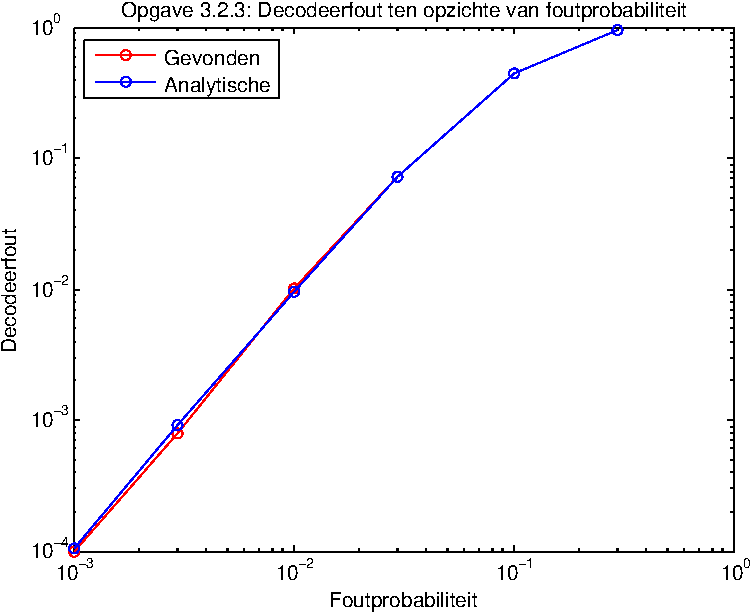
\includegraphics[width=0.8\textwidth]{3_2_3_foutprob.pdf}
  		\caption{Opgave 3.2.3: Decodeerfout ten opzichte van foutprobabiliteit}
  		\label{fig:3_2_3_foutprob}
\end{figure}

\begin{table}
\centering
\begin{tabular}{l|l|l}
Kans p & Analytische decodeerfoutkans & Decodeerfoutkans simulatie \\
\hline
0.3		& 0.964732    & 0.9641 \\
0.1		& 0.450957    & 0.4489 \\
0.03	& 0.0729725   & 0.0733 \\
0.01	& 0.00962977  & 0.0102 \\
0.003	& 0.000920759 & 0.0008 \\
0.001	& 0.000104094 & 0.0001 \\
\end{tabular} 
\caption{Tabel met de verwachte en gevonden decodeerfoutkansen voor een informatiewoord voor vraag 3 uit kanaalcodering.}
\label{tab:1.6}
\end{table}

We zien zowel grafisch als in de tabel dat de berekende decodeerfoutkansen zeer dicht bij de praktisch bekomen decodeerfoutkansen liggen.


\subsection{Productcode \texttt{Prod\_encode$\left(\right)$}}

De productcode zal op ieder blok van $l$ codewoorden \texttt{Ham\_Encode} toepassen. Aan het resultaat hiervan zal een extra rij met voor iedere kolom een pariteitsbit toegevoegd worden.\\

De minimale hammingafstand van de productcode is het product van de minimale hammingafstanden van de beide foutcorrigerende codes gebruikt om de productcode te construeren. De eerste code heeft een minimale hammingafstand 3, de tweede code die enkel een pariteitsbit zal toevoegen heeft een minimale hammingafstand 2. We bekomen dus dat de minimale hammingafstand van de productcode 6 is.

\subsection{Implementatie Decoder en oncorrigeerbare foutpatronen}
Het implementeren van de decoder is helaas niet gelukt. Bij het testen krijgen we een afbeelding terug, maar bestaat enkel maar uit ruis. Deze is te zien op figuur \ref{fig:3_2_7_3_fout} op pagina \pageref{fig:3_2_7_3_fout}. Hoewel we lang op de fout hebben gezocht hebben we deze niet gevonden.

\begin{figure}[h!]
  		\centering
   		
\includegraphics[width=0.4\textwidth]{3_2_7_3.pdf}
  		\caption{Foute afbeelding, ge-encodeerd en gedecodeerd met de productcode}
  		\label{fig:3_2_7_3_fout}
\end{figure}

We kunnen twee gevallen beschouwen waar oncorrigeerbare foutpatronen voorkomen.
Ten eerste is er het geval dat er een pariteitsbit omflipt en op dezelfde rij er een syndroom verschillend van nul is. In dat geval gaan we een bit verbeteren terwijl dit mogelijks niet nodig is. \\
Ten tweede is er het geval dat er een even aantal ( maar meer dan 2 ) rijen een fout staat in dezelfde kolom waarvan de pariteitsbits nog juist zijn. In dat geval zal de pariteitscheck kloppen en zullen deze fouten niet verbeterd worden. 

\subsection{Bepaling decodeerfout bij productcode adhv simulaties}

De kans dat er in 8 codewoorden minstens 1 decodeerfout optreedt is gegeven door volgende formule:
\begin{equation*}
1 - Pr[\text{kans op fout in de hammingcode}]^8 = 1 - ((1-p)^{15}+15p(1-p)^{14})^8
\end{equation*}
De bekomen resultaten zijn te zien in tabel \ref{tab:1.7} op pagina \pageref{tab:1.7}. Aangezien de functie \texttt{prod\_decode} niet werkt hebben we de decodeerfoutkansen niet kunnen simuleren.

\begin{table}[h!]
\centering
\begin{tabular}{l|l|l}
Kans p & Analytische decodeerfoutkans & Decodeerfoutkans simulatie\\
\hline
0.3		&	$\approx$ 1  & / \\
0.1		& 0.99174    & / \\
0.03	& 0.45468    & / \\
0.01	& 0.074491   & / \\
0.003	& 0.0073424  & / \\
0.001	& 0.00083245 & /
\end{tabular} 
\caption{Tabel met de verwachte en gevonden decodeerfoutkansen voor een blok van 8 informatiewoorden voor vraag 6 uit kanaalcodering.}
\label{tab:1.7}
\end{table}

De analytische foutkansens hebben we nog eens visueel voorgesteld in figuur \ref{fig:3_2_6_foutprob} op pagina \pageref{fig:3_2_6_foutprob}. Hier hebben we de waarden uit de tabel voor de productcode nog eens door 8 gedeeld om de foutkans per informatiewoord te krijgen in plaats van per blok. We zien duidelijk dat de productcode beter presteert dan de Hammingcode.

\begin{figure}[h!]
  		\centering
   		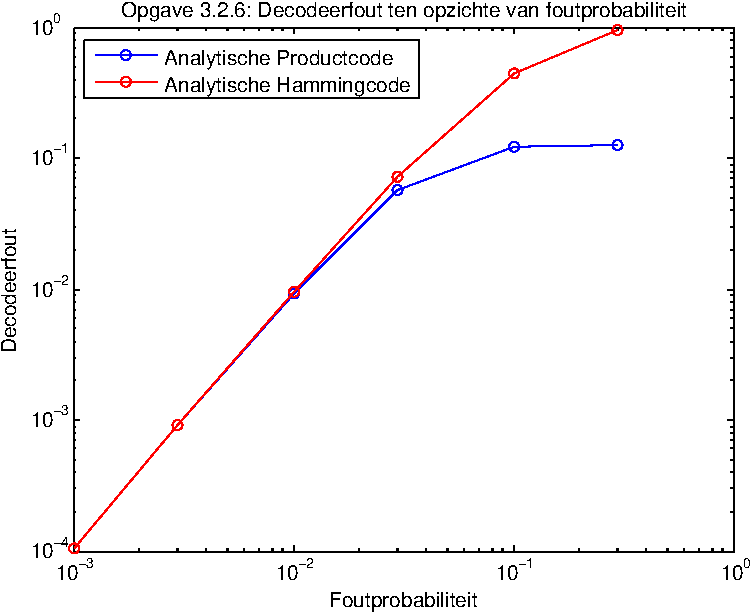
\includegraphics[width=0.8\textwidth]{3_2_6_foutprob.pdf}
  		\caption{Opgave 3.2.6: Analytische decodeerfout Hammingcode ten opzichte van analytische decodeerfout productcode}
  		\label{fig:3_2_6_foutprob}
\end{figure}


\subsection{Verschillen tussen verstuurde afbeeldingen}
De verkregen afbeeldingen zijn te zien in figuur \ref{fig:7_verk_afb} op pagina \ref{fig:7_verk_afb}. De derde afbeelding hebben we niet kunnen opstellen aangezien het decoderen met de productcode niet werkt.

\paragraph*{Gecodeerde transmissie}
Bij de niet gecodeerde transmissie zien we duidelijk dat er redelijk wat fouten voorkomen en dat deze fouten gelijkmatig verspreid zijn over de gehele afbeelding. Dit is te wijten aan de foutprobabiliteit van het kanaal. 

\paragraph*{Gecodeerde transmissie met Hammingcode} Door het toepassen van de Hammingcode zal het aantal fouten beperkt worden. We zien ook dat ze gelokaliseerd zijn.

\paragraph*{Gecodeerde transmissie met Productcode} Door de grotere Hammingafstand van de productcode zullen er hier nog minder fouten optreden. We verwachten dus dat we een bijna foutloze afbeelding krijgen.

\begin{figure}[h!]
        \centering
\begin{subfigure}[b]{0.35\textwidth}
  		\centering
   		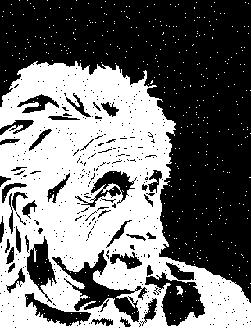
\includegraphics{3_2_7_1.pdf}
  		\caption{Niet gecodeerde transmissie}
  		\label{fig:3_2_7_1}
\end{subfigure}
\begin{subfigure}[b]{0.35\textwidth}
  		\centering
   		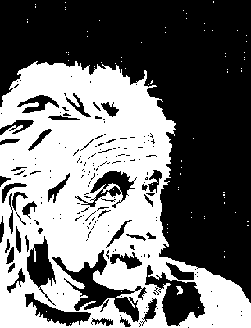
\includegraphics{3_2_7_2.pdf}
  		\caption{Gecodeerde transmissie met hammingcode}
  		\label{fig:3_2_7_2}
\end{subfigure}		
  		\caption{Verkregen afbeeldingen}\label{fig:7_verk_afb}
\end{figure}



\section{Volledig systeem}
\subsection{Ontvangen afbeeldingen}
De verkregen afbeeldingen zijn te zien in figuur \ref{fig:8_verk_afb} op pagina \ref{fig:8_verk_afb}. De code gebruikt om deze op te stellen is terug te vinden in het bestand \texttt{3.m}. Ook hier hebben we de laatste afbeelding niet kunnen opstellen.

\begin{figure}[h!]
        \centering
\begin{subfigure}[b]{0.33\textwidth}
  		\centering
   		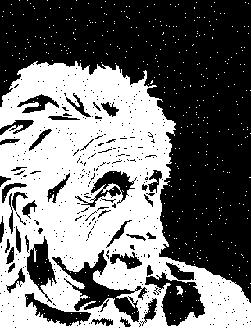
\includegraphics{3_3_1.pdf}
  		\caption{Transmissie zonder codering en compressie}
  		\label{fig:3_3_1}
\end{subfigure}
\begin{subfigure}[b]{0.33\textwidth}
  		\centering
   		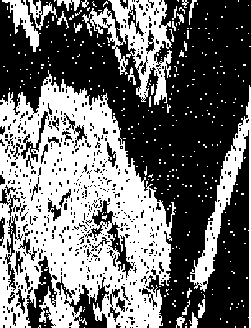
\includegraphics{3_3_2.pdf}
  		\caption{Gecomprimeerde transmissie}
  		\label{fig:3_3_2}
\end{subfigure}	
  		\caption{Verkregen afbeeldingen}\label{fig:8_verk_afb}
\end{figure}

\subsection{Bespreking verschillen}

\paragraph*{Transmissie zonder codering en compressie} We zien dat er een aantal fouten zijn opgetreden en dat deze fouten gelijkmatig verspreid zijn over de hele afbeelding. Dit is te wijten aan de foutprobabiliteit van het kanaal. 

\paragraph*{Gecomprimeerde transmissie} In deze afbeelding kunnen we nog steeds vanuit de verte de vorm van Einstein herkennen. Wat opvalt is dat de hele afbeelding er `verschoven' uit ziet. Dit is als volgt te verklaren: Stel dat we een alfabet hebben van 0, 1 met als bijhorende codes 0 en 10. Als we als input nu de string `1100' krijgen, 4 bits dus, encoderen we dit als `101000'. Stel nu dat we deze ge-encodeerde string versturen over een kanaal en we krijgen aan de andere kant van dit kanaaal de string `101010' terug. Bij het decoderen krijgen we nu niet `1100' maar `111'. Dit zijn geen 4 bits zoals oorspronkelijk, maar 3.\\
Dit is exact hetzelfde wat gebeurt bij de afbeelding, maar dan op grotere schaal. Dit uit zich in de figuur als verschuiving.

\paragraph*{Gecomprimeerde en gecodeerde transmissie met de productcode} We verwachten hier een gelijkaardig verschuivingseffect te zien zoals in de vorige afbeelding maar veel minder extreem. Dit komt omdat de productcode de meeste fouten zal opvangen en corrigeren, maar nog niet alle.

\end{document}